
\begin{figure}[!h]
\centering
\includegraphics[width=\textwidth]{Modules/Picture/Utilisation.png}
\caption{Ecriture et acquisition}
\label{utilisation}
\end{figure}

Ce dispositif nous permet de capturer les vidéos en direct. Ces deux vidéos sont enregistrées sur ordinateur, pour pouvoir faire de la stéréo : on encode les images en même temps pour avoir exactement les mêmes frames au même moment. On applique ensuite des paramètres d'undistortion pour lisser les bords de l'image. En effet, la caméra ayant un grand angle, l'extérieur de l'image est déformé, ce qui peut apporter des problèmes lors de la reconstruction 3D.

Une fois les deux vidéos récupérées, on peut lancer la reconstruction. La première étape est de retrouver l'écriture sur l'image, pour cela différentes méthodes sont disponibles. Comme sur la figure \ref{tracking}, on peut faire du tracking. Après avoir sélectionné une zone d'intérêt grâce à un ROI (Region Of Interest) selector (figure \ref{ROI} ), on essaye de suivre le mouvement. Il suffit d'enregistrer les coordonnées du centre du point pour retrouver le mouvement dessiné.

La seconde technique est celle du HOG (Histogramme de gradient orienté) qui permet de détecter des formes dans une image. Ce qui donne au départ une image comme sur la figure \ref{HOGSale}, et après nettoyage \ref{HOGPropre}.

L'une ou l'autre de ces techniques peuvent être utilisés pour avoir une suite de coordonnées correspondant au dessin de l'écriture. Une fois que ces deux coordonnées sont récupérées, il existe des fonctions dans OpenCV pour faire des points 3D à partir de points 2D. Il faut pour cela récupérer les paramètres extrinsèques (matrices de rotation et vecteurs de translation, pour passer du repère lié à l'espace de travail au repère lié à la caméra) de la caméra.

Une fois que les coordonnées sont récupérées par l'une ou l'autre méthode, une fonction nous permet de rajouter deux points entre chaque coordonnées pour fluidifier la ligne. Ces coordonnées sont ensuite interprétées par OpenGL pour permettre de les afficher dans un repère en trois dimensions (figures \ref{3D1} et \ref{3D2} ).


\begin{figure}[htb]
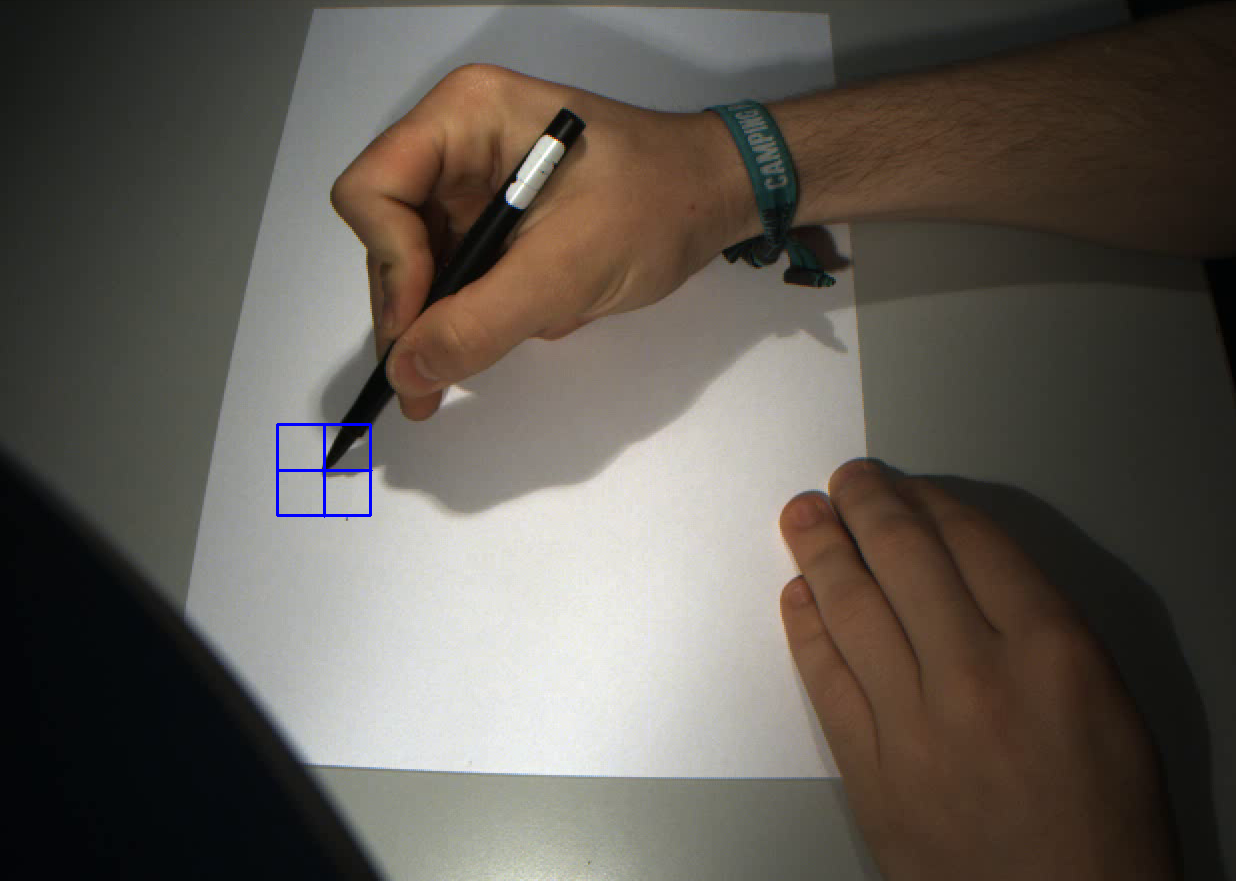
\includegraphics[width=\textwidth]{Modules/Picture/roi}
\caption{ROI selector}
\label{ROI}
\vspace{30px}
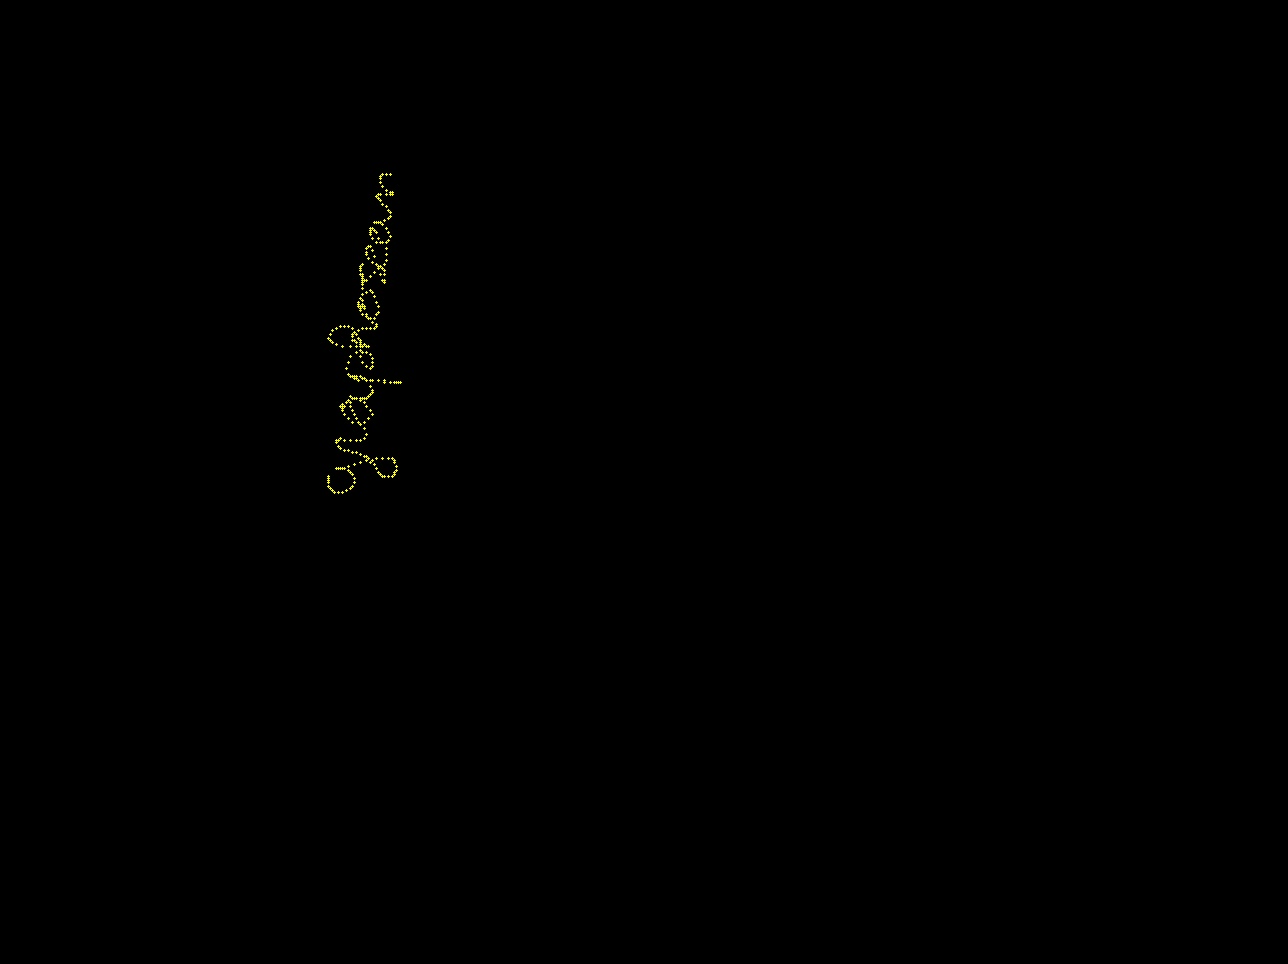
\includegraphics[width=\textwidth]{Modules/Picture/tracking}
\caption{Reconnaissance avec le tracking}
\label{tracking}
\end{figure}

\newpage

\begin{figure}
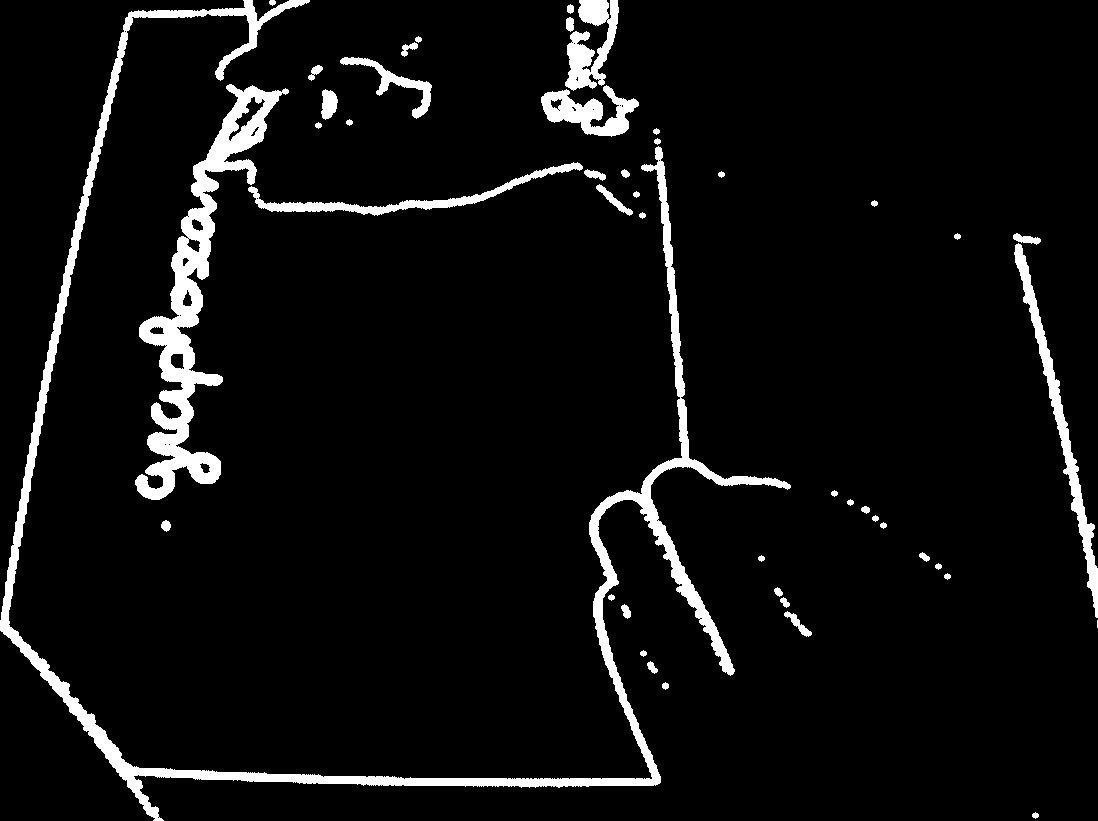
\includegraphics[width=\textwidth]{Modules/Picture/hog}
\caption{HOG brut}
\label{HOGSale}
\vspace{30px}
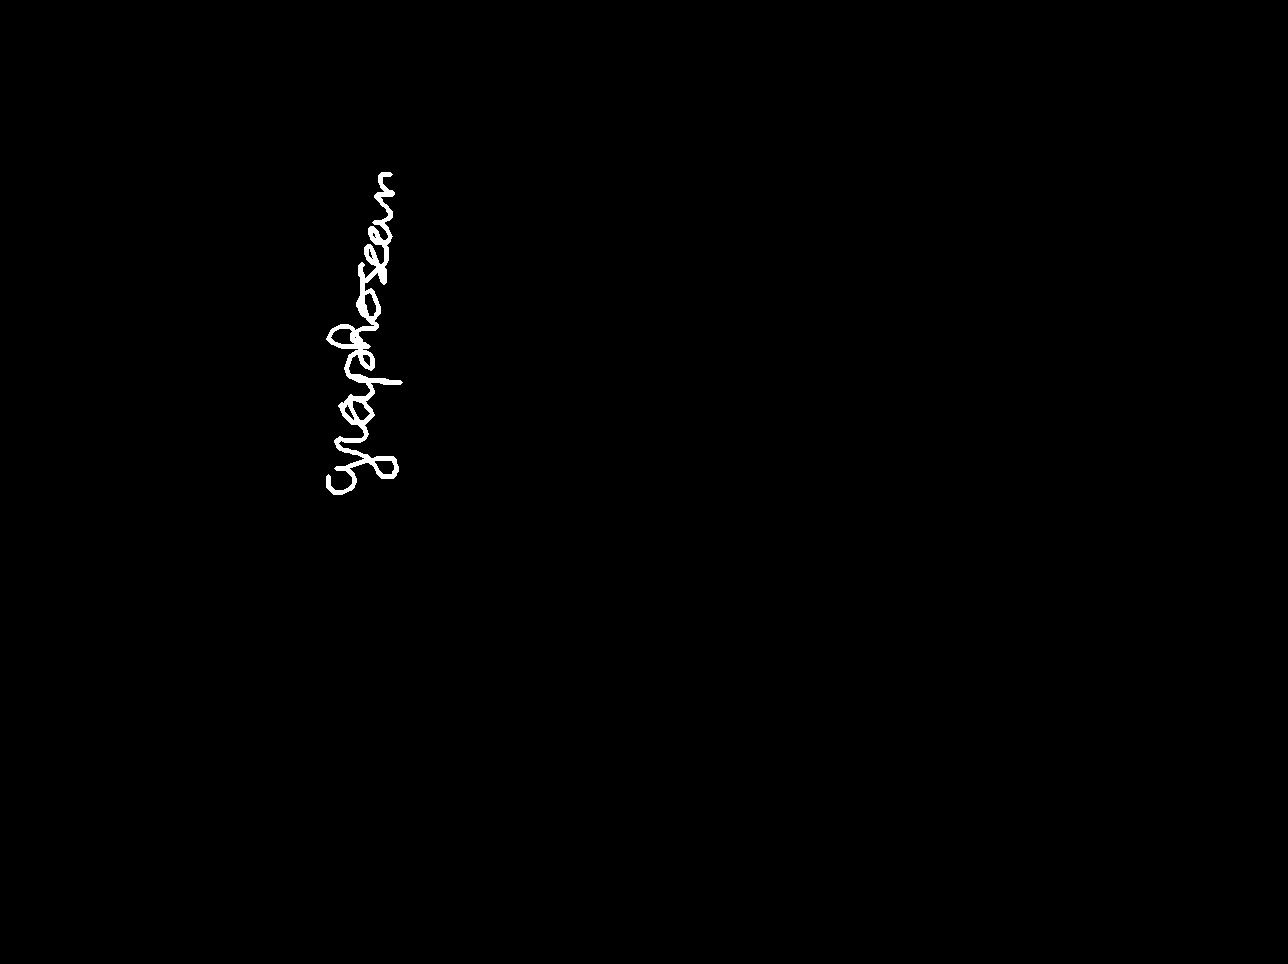
\includegraphics[width=\textwidth]{Modules/Picture/hog_propre}
\caption{HOG nettoyé}
\label{HOGPropre}
\end{figure}

\newpage

\begin{figure}
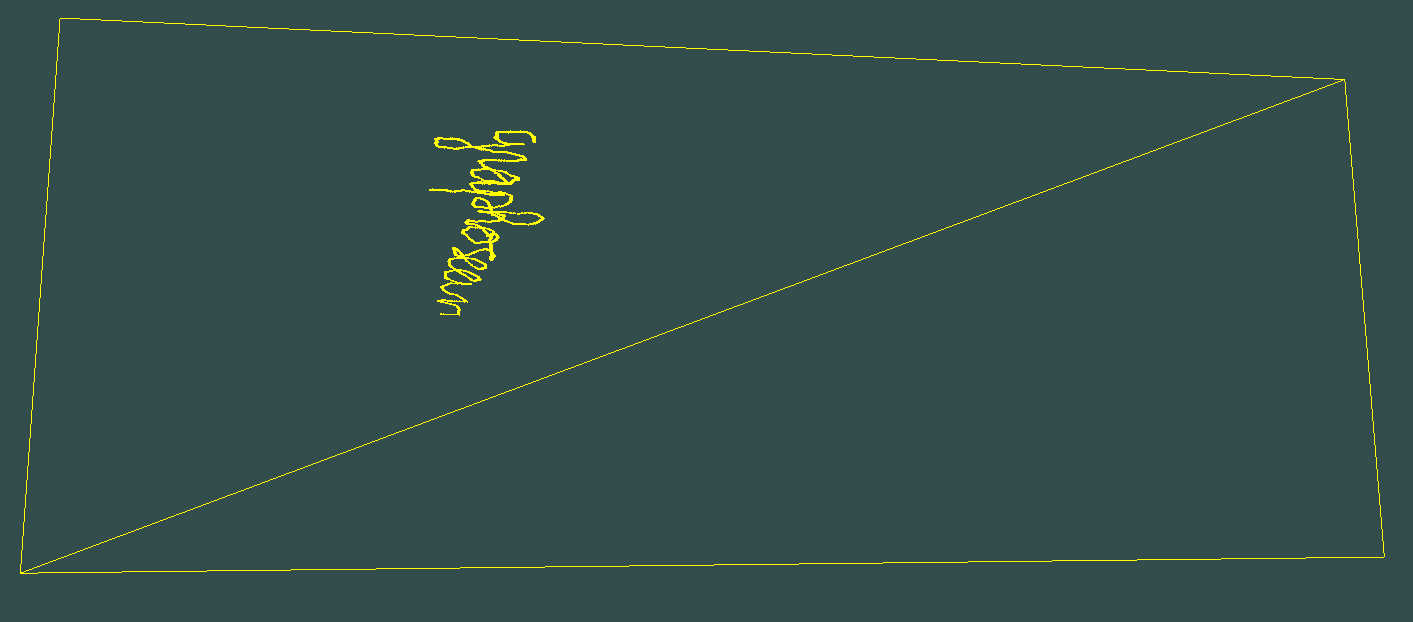
\includegraphics[width=\textwidth]{Modules/Picture/3d_1}
\caption{Image 3D - 1}
\label{3D1}
\vspace{30px}
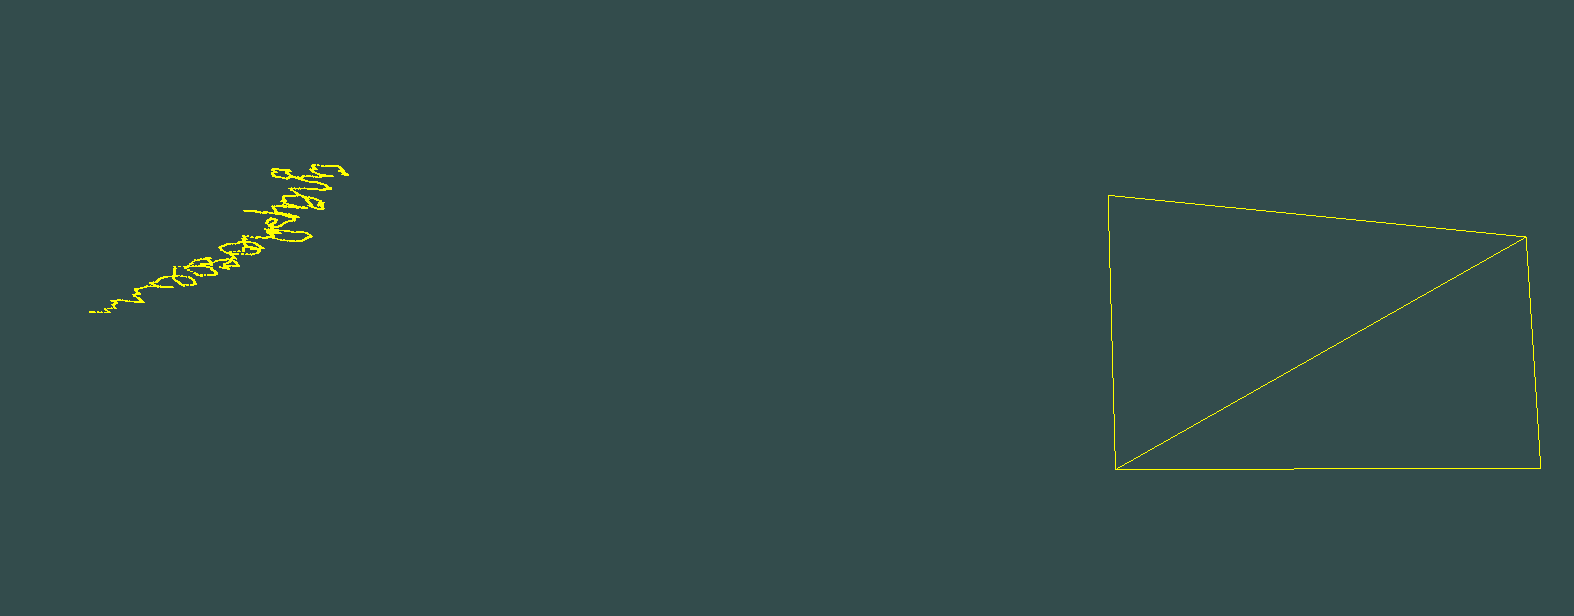
\includegraphics[width=\textwidth]{Modules/Picture/3d_2}
\caption{Image 3D - 2}
\label{3D2}
\end{figure}

\clearpage